\documentclass[liststotoc,bibtotoc,fontsize=14pt,]{scrreprt}
\usepackage[utf8]{inputenc} % Zeichenkodierung
\usepackage[ngerman]{babel} % neue deutsche Rechtschreibung
\usepackage{etoolbox}
\setlength{\footskip}{30pt}
\apptocmd{\thebibliography}{\raggedright}{}{}
\usepackage{graphicx}
\usepackage{caption}
\usepackage{subcaption}
\usepackage{url}
\usepackage[onehalfspacing]{setspace}
\usepackage{breakurl}
\usepackage{float}
\usepackage[table,xcdraw]{xcolor}
\usepackage{tabularx}
\usepackage[breaklinks]{hyperref}
\def\UrlBreaks{\do\/\do-}
\usepackage{tocloft}
\usepackage{chngcntr}
\usepackage{listings}
\usepackage{color}
\usepackage[parfill]{parskip}
\definecolor{lightgray}{rgb}{.9,.9,.9}
\definecolor{darkgray}{rgb}{.4,.4,.4}
\definecolor{purple}{rgb}{0.65, 0.12, 0.82}

\counterwithout{footnote}{chapter}

\deffootnote[2em]{2em}{2em}{%
	\makebox[2em][l]{\bfseries\thefootnotemark}}

\renewcommand{\cftchapdotsep}{\cftdotsep}
\renewcommand{\cftchapleader}{\cftdotfill{\cftchapdotsep}}
\usepackage{amsmath}
\usepackage[paper=a4paper,left=30mm,right=30mm,top=25mm,bottom=25mm]{geometry}
\usepackage[section]{placeins}
\usepackage[font=small,justification=justified]{caption}
\newcommand{\namesigdate}[3][Ort, Datum]{%
	\parbox{\textwidth}{
		\raggedleft #3 
		\vspace{2cm}
		
		\parbox{5cm}{
			\raggedright
			\rule{6cm}{1pt}\\
			#1 
		}
		\hfill
		\parbox{5cm}{
			\raggedright
			\rule{6cm}{1pt}\\
			#2
		}
	}
}


\newcommand*{\tabularwidth}{}
\newdimen\tabularwidth
\usepackage{minitoc}
\hypersetup{
	colorlinks,
	citecolor=black,
	filecolor=black,
	linkcolor=black,
	urlcolor=black
}


\title{Dokumentation Panoramafotografie}
\author{Sebastian Degner}

\begin{document}
	%\maketitle
	
	\begin{titlepage}
		\begin{center}
			\vspace{2cm}
			Dokumentation\\ \textbf{Multishot-Technik in der digitalen Fotografie}\\ 
			\vspace{2,5cm}
			
\includegraphics[width=5cm]{HTWK_Logo_RGB-transparent_250.png}\\
			
			\vspace{2,5cm}
			\huge \textbf{\textsf{Dokumentation HDR-Fotografie}} \\
			\vspace{3cm}
			\fontsize{15}{18} \textbf{Hochschule für Technik, Wirtschaft und Kultur
				Leipzig\\ Fakultät Informatik, Mathematik und Naturwissenschaften\\   Masterstudiengang Medieninformatik}\\
			\vspace{3cm}
		\end{center}
		\normalsize{
			\begin{tabular}{ll}
				Eingereicht von: & {Sebastian Degner} \\
				 & {Sebastian Knabe} \\
				Studiengang: & 15 MIM\\
				Eingereicht am: & 31. Januar 2017 \\
			\end{tabular}\\
		}
		
	\end{titlepage}
	
	\tableofcontents
	\clearpage
	\listoffigures
	\addcontentsline{toc}{chapter}{Abbildungsverzeichnis}

	\chapter{Einleitung}
	\label{ch:einleitung}
	Im Rahmen des \textit{Moduls Multishot-Technik in der digitalen Fotografie} wurde diese Dokumentation zu dem Thema \textit{High Dynamic Range} (auch mit HDR abgekürzt) realisiert. Mit Hilfe der HDR-Fotografie lassen sich Aufnahmen erstellen, welche einen besonders hohen Kontrastumfang aufweisen. Fotos, welche mit dieser Technik aufgenommen werden Helligkeitsunterschiede detailreich wiedergeben. Außerdem wird vermieden, das Bildinformation durch Über- beziehungsweise Unterbelichtung verloren gehen. HDR-Aufnahmen können mit  einer handelsüblichen Spiegelreflexkamera nicht direkt aufgenommen werden. Um diese zu erzeugen muss man mehrere Einzelbilder aufnehmen, welche später mit Hilfe spezieller Software zu einem HDR-Foto zusammengefügt werden.
	
	\bigskip
	Im Verlauf dieser Arbeit wird detailliert gezeigt, wie die insgesamt sechs HDR-Aufnahmen entstehen. Dabei werden sowohl die  Kameraeinstellungen, als auch die verwendete Software beschrieben. 
		
	\chapter{Aufnahmen}
	\label{ch:aufnahmen}
	
	\section{Leipziger Baumwollspinnerei}
	\label{sec:spinnerei}

	\subsubsection{Aufnahmeort und -idee}
	Die Leipziger Baumwollspinnerei wurde 1884 gegründet und noch im gleichen Jahr wurde im Leipziger Westen die erste Spinnerei (Heute Halle 20) eröffnet. Der Bedarf an Baumwolle war damals so hoch, dass die Leipziger Baumwollspinnerei innerhalb weniger Jahre zur größten Europas wurde. Nach und nach entstand eine Fabrikstadt mit insgesamt 20 Produktionsgebäuden, Arbeiterwohnungen und Kindergärten. Auf dem Höhepunkt hatte die Leipziger Baumwollspinnerei eine Größe von 100.000m$^2$ und beschäftigte bis zu 4000 Mitarbeiter. Die Produktion wurde nach der Wiedervereinigung eingestellt.
	
	\bigskip
	Revitalisiert wurde die Baumwollspinnerei vorallem durch die Kunstszene Leipzigs. Heute sind viele Gebäude des Geländes saniert und die Leipziger Baumwollspinnerei dass Zentrum der Leipziger Kunstszene. Dort finden sich unter anderem elf Galerien und ein gemeinnütziges Kunstzentrum. Der architektonische Kontrast zwischen Alt und Neu macht den besonderen Reiz dieses Ortes aus.
		\begin{figure}[H]
			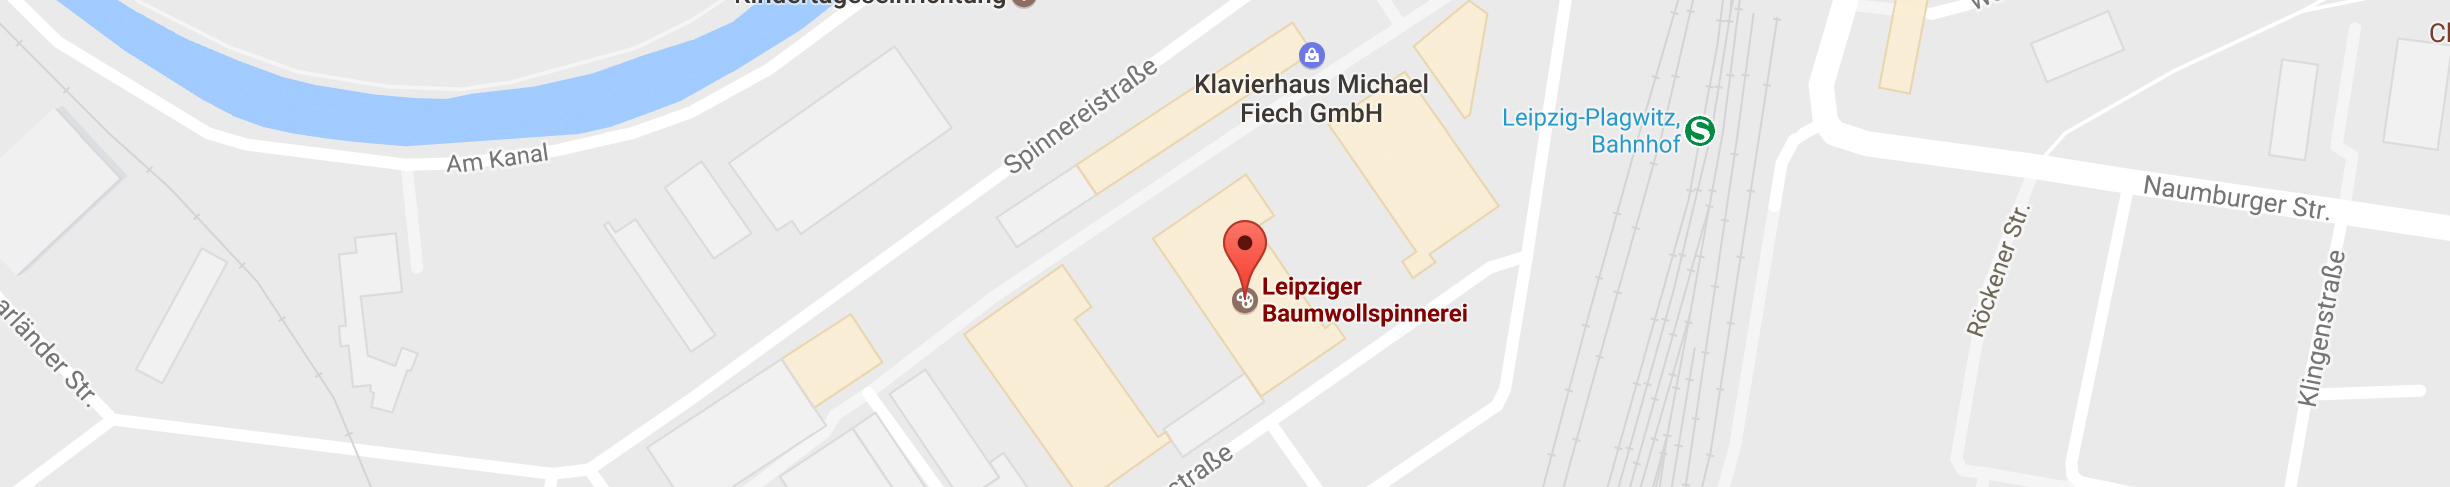
\includegraphics[width=\linewidth]{img/places/spinnerei_map.jpg}
			\caption{Aufnahmeort Baumwollspinnerei}
			\label{img:ak_map}
		\end{figure}

		\subsubsection{Kameraeinstellungen}
			\begin{minipage}{0.58\textwidth}
				\begin{tabular}{ll}
					Kamera: &Canon EOS 7D \\
					Objektiv: &Canon EF 10-22mm \\
					& F/3.5-4.5 USM\\		
					Brennweite:& 10mm \\
					Belichtungszeit: & $\frac{1}{30}$s /$\frac{1}{15}$s /$\frac{1}{4}$s / $\frac{1}{2}$s \\
					 & 1s\\
					Blendenwert: & f/8\\
					Empfindlichkeit & ISO 100 \\
				\end{tabular}\\
			\end{minipage}%
			\begin{minipage}{0.42\textwidth}
				\begin{figure}[H]
					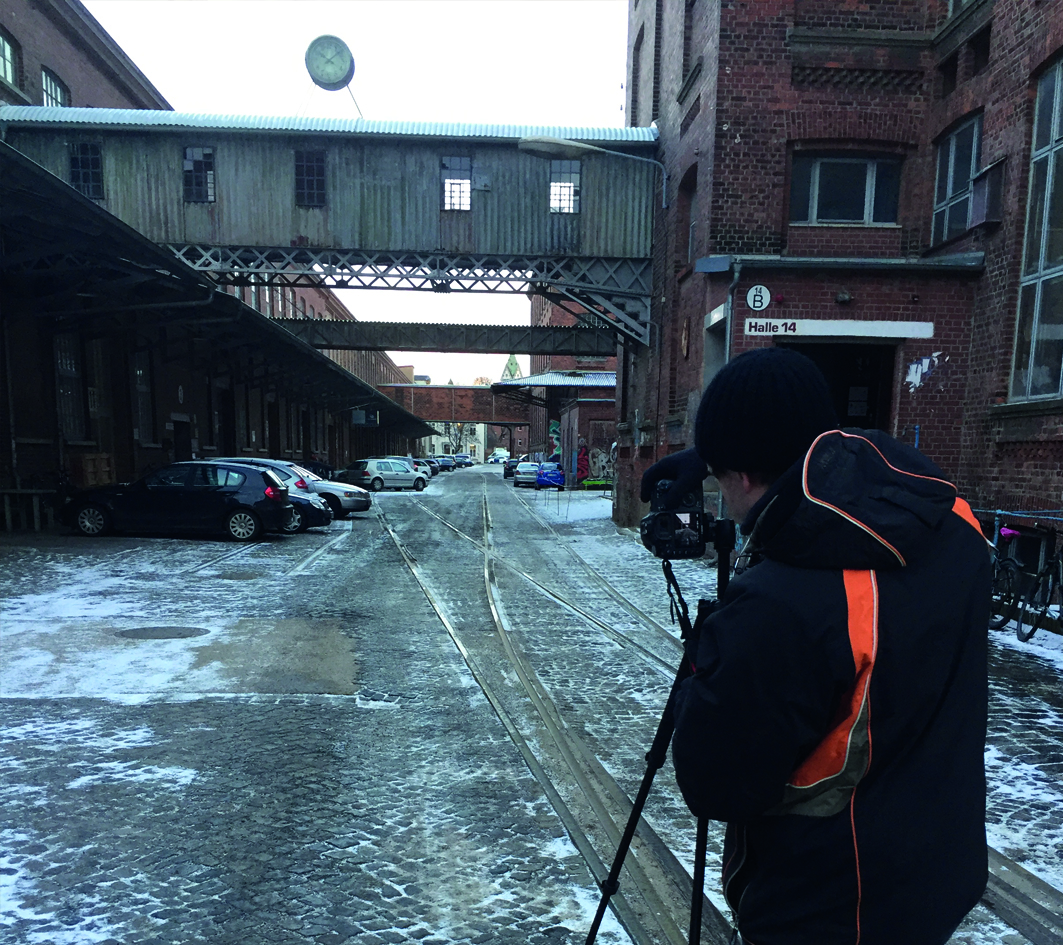
\includegraphics[width=\linewidth]{img/places/spinnerei.jpg}
					\caption{Aufnahmesituation Baumwollspinnerei}
					\label{img:ak}
				\end{figure}
			\end{minipage}%

	\subsubsection{Vorgehen}
	Es wurden fünf Einzelbilder aufgenommen, welche später mit Hilfe geeigneter Software zu einer HDR-Aufnahme zusammengefügt werden. Die Bilder entstanden am 05.01.2017 um 16:00 Uhr. Als Motiv wurde die Überführung, das Wahrzeichen der Leipziger Baumwollspinnerei gewählt. 
	
	\newpage
	\begin{figure}[h]
		
\includegraphics[width=\linewidth]{img/ph.jpg}
		\caption{HDR-Aufnahme Leipziger Baumwollspinnerei}
	\end{figure}

\section{Palmengarten Leipzig}
\label{sec:palme}
\subsubsection{Aufnahmeort und -idee}
Der Leipziger Palmengarten befindet sich am westlichen Ende der Jahnallee und zwei Kilometer südwestliche der Leipziger Innenstadt. Ursprünglich befand sich an dieser Stelle ein Teil des Auwaldes, bis im Jahr 1893 geplant wurde einen Palmengarten nach Vorbild des Frankfurter Palmengartens zu schaffen. Nach einer öffentlichen Ausschreibung wurde dieser schließlich 1899 eröffnet und als vornehmste Erholungsstätte Leipzigs betitelt. Neben einer Parkanlage wurde auf dem Gelände auch ein Palmenhaus errichtet, welches der Namensgeber der Anlage war. Dieses wurde allerdings 1939 gesprengt und der anschließende zweite Weltkrieg verhinderte die Neuerrichtung des Gebäudes. 

\bigskip
Heute befindet sich an dieser Stelle unter anderem eine kleine Anlage, welche sich vorallem durch ihren Stufenartigen Aufbau vom restlichen Park abhebt. Besonders markant sind die massiven Pflanzenranken, welche im Zusammenspiel mit der, zu der Zeit als die Aufnahmen entstanden sind, vorherrschenden Winterlandschaft und den Bäumen im Hintergrund einen starken Kontrast bilden und somit für die Realisierung einer HDR-Aufnahmen sehr gut geeignet sind. 

\begin{figure}[H]
	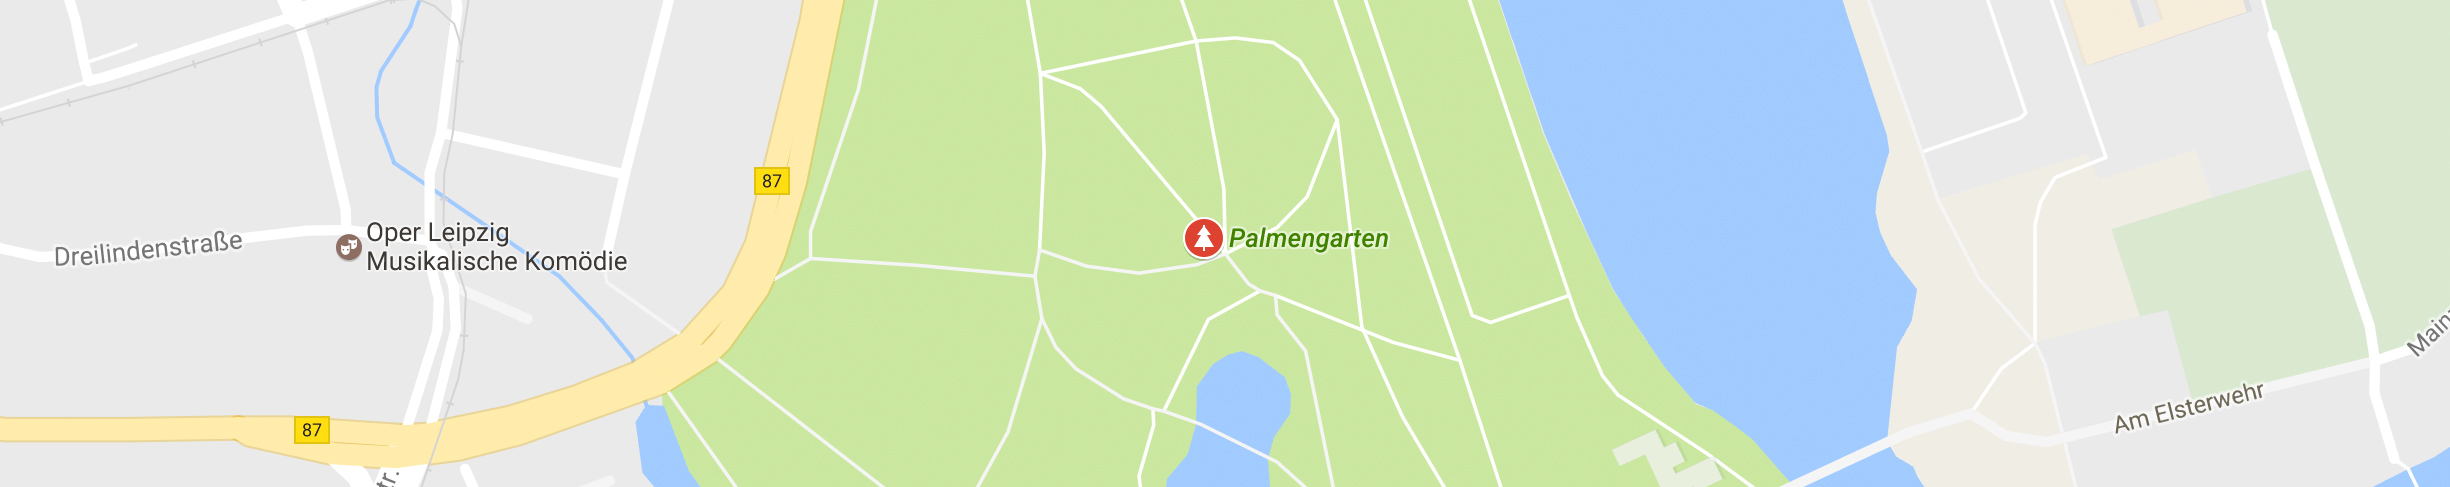
\includegraphics[width=\linewidth]{img/places/palmen_map.jpg}
	\caption{Aufnahmeort Palmengarten Leipzig}
	\label{img:ak_map}
\end{figure}

\subsubsection{Kameraeinstellungen}
\begin{minipage}{0.58\textwidth}
	\begin{tabular}{ll}
		Kamera: &Canon EOS 7D \\
		Objektiv: &Canon EF 10-22mm \\
		& F/3.5-4.5 USM\\		
		Brennweite:&  10mm \\
		Belichtungszeit: & $\frac{1}{30}$s /$\frac{1}{15}$s /$\frac{1}{8}$s / $\frac{1}{4}$s \\
		& $\frac{1}{2}$s \\
		Blendenwert: & f/8\\
		Empfindlichkeit & ISO 100\\
	\end{tabular}\\
\end{minipage}%
\begin{minipage}{0.42\textwidth}
	\begin{figure}[H]
		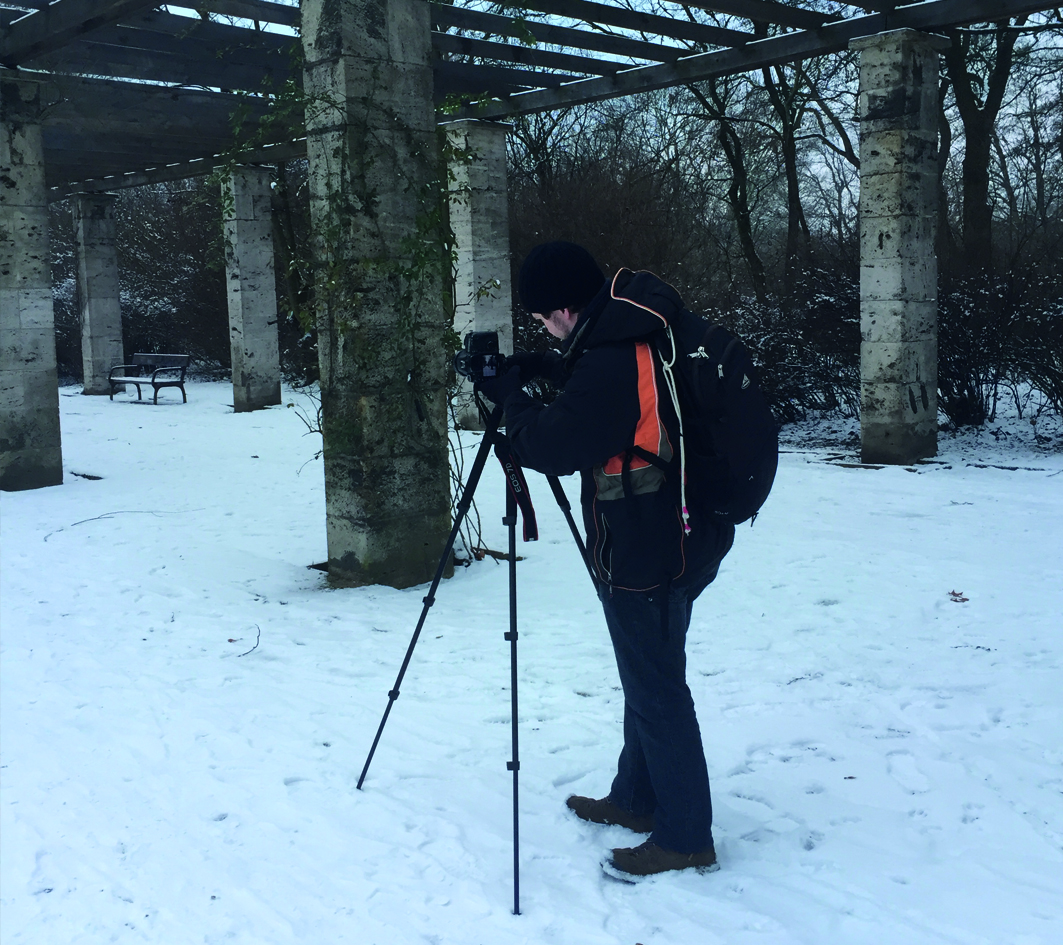
\includegraphics[width=\linewidth]{img/places/palmen.jpg}
		\caption{Aufnahmesituation Palmengarten Leipzig}
		\label{img:ak}
	\end{figure}
\end{minipage}%


\subsubsection{Vorgehen}
Die Aufnahmen entstanden am 17.01.2017 um 16:03 Uhr. Die Kamera wurde seitlich der Pflanzenranken positioniert, sodass diese zwar das vorherrschende Motiv sind, aber die Umgebung, wie beispielsweise Bäume dennoch mit aufgenommen werden konnten. Die optischen Linien der Pflanzenranken, sowie des Weges lenken gewollt den Blick des Betrachters und vereinen sich ein einem gemeinsamen Fluchtpunkt.

\newpage
\begin{figure}[h]
	
\includegraphics[width=\linewidth]{img/ph.jpg}
	\caption{HDR-Aufnahme Palmengarten Leipzig}
\end{figure}

\section{Nikolaikirche}
\label{sec:nikolai}
\subsubsection{Aufnahmeort und -idee}
Die Nikolaikirche ist die größte Kirche Leipzigs und neben der Thomaskirche auch eine der bekanntesten, da von ihr die Montagsdemonstrationen und somit schließlich die friedliche Revolution ausging. Benannt ist sie nach dem heiligen Nikolaus und bildet das Zentrum der evangelisch-lutherischen Kirchengemeinde Leipzigs. Im Jahr 1165 wurde die Nikolaikirche im romanischen Stil, welcher bis heute an der Westseite der Kirche noch erkennbar ist, erbaut. Während der Zeit der Aufklärung wurde der Innenraum nach Vorbild der \textit{Urhütte} umgestaltet, sodass die zahlreichen Säulen im Innenraum an Bäume erinnern sollen. 

\bigskip
Eine dieser Säulen befindet sich Heute auch außerhalb der Nikolaikirche, auf dem Kirchhof und bildet zusammen mit der Kirche im Hintergrund das Motiv dieser HDR-Fotografie.

\begin{figure}[H]
	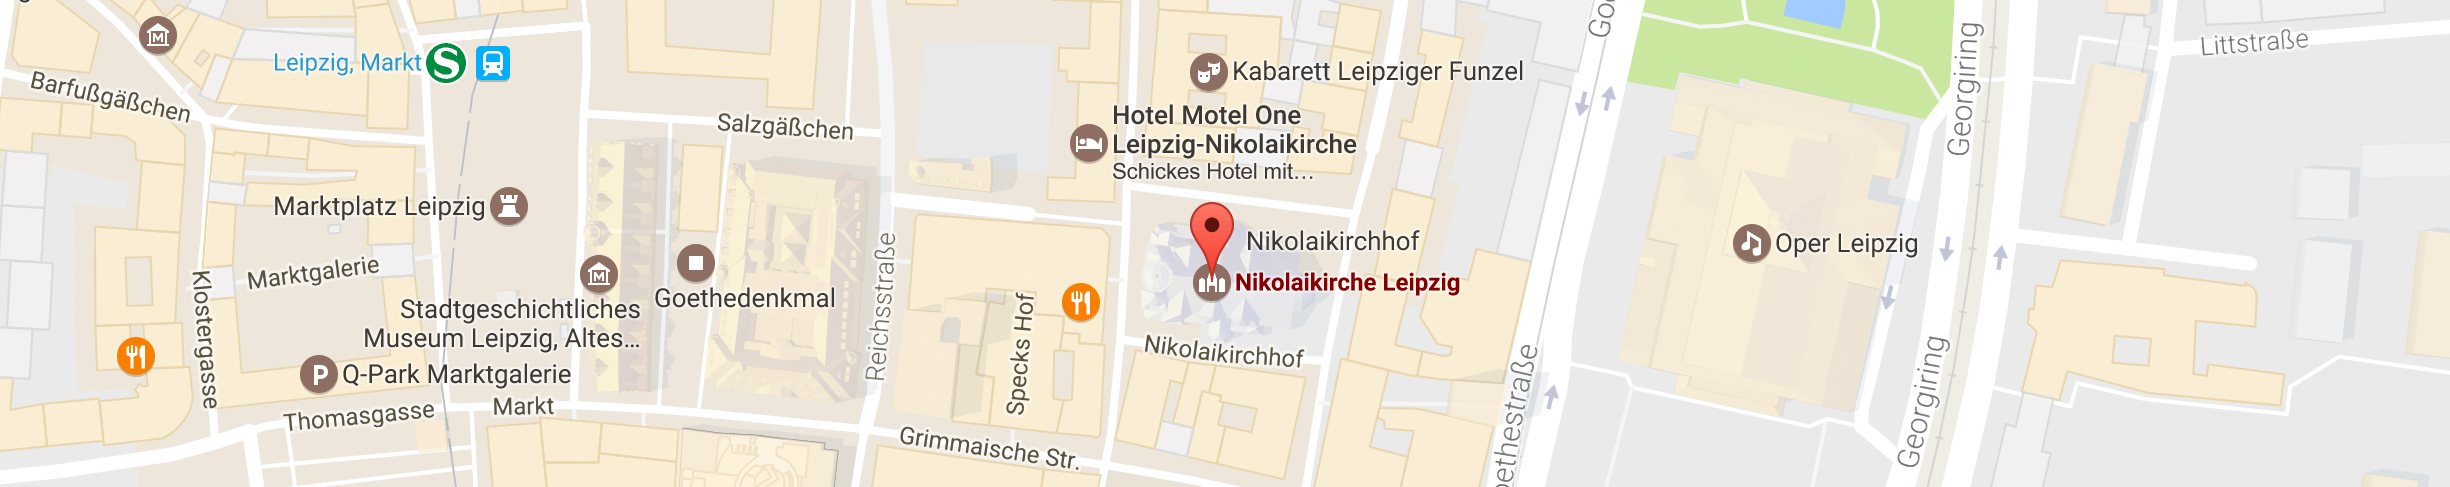
\includegraphics[width=\linewidth]{img/places/nikolai_map.jpg}
	\caption{Aufnahmeort Nikolaikirche}
	\label{img:ak_map}
\end{figure}

\subsubsection{Kameraeinstellungen}
\begin{minipage}{0.58\textwidth}
	\begin{tabular}{ll}
		Kamera: &Canon EOS 7D \\
		Objektiv: &Canon EF 10-22mm \\
		& F/3.5-4.5 USM\\		
		Brennweite:&  10mm \\
		Belichtungszeit: & 1s / 2s / 4s / 8s / 15s \\
		Blendenwert: & f/8\\
		Empfindlichkeit & ISO 100\\
	\end{tabular}\\
\end{minipage}%
\begin{minipage}{0.42\textwidth}
	
\end{minipage}%

\subsubsection{Vorgehen}
Für die Realisierung dieser HDR-Fotos wurden die Einzelbilder am 17.01.2017 um 16:48 Uhr aufgenommen. Zu dieser Uhrzeit setzt die Dämmerung gerade ein, sodass die umliegenden Geschäfte, Gebäude, sowie Teile der Nikolaikirche bereits beleuchtet sind, aber der Himmel dennoch samt seiner Strukturen hell und klar erkennbar ist.  Die Kamera wurde so platziert, dass sie sowohl die Säule in ihrer Höhe, als auch Kirche in ihrer Breite komplett ablichtet. Auf Grund der engen Bebauung und des damit einhergehenden begrenzten Platzes wurde ein Weitwinkelpbjektiv verwendet. 
\newpage
\begin{figure}[h]
	
\includegraphics[width=\linewidth]{img/ph.jpg}
	\caption{HDR-Aufnahme Nikolaikirche}
\end{figure}
	
	\section{City-Tunnel Wilhelm-Leuschner-Platz }
	\label{sec:tunnel}
	\subsubsection{Aufnahmeort und -idee}
	Der Wilhelm-Leuschner-Platz befindet sich am südlichen Ende des Leipziger Innenstadtrings. Benannt wurde er nach dem Gewerkschafter und sozialdemokratischen Politiker Wilhelm Leuschner, welcher von 1890 bis 1944 lebte. Heute befindet sich auf dem Platz ein Knotenpunkt für den öffentlichen Personennahverkehr, welcher 2013 mit der Fertigstellung des City-Tunnels weiter ausgebaut wurde. 
	
	\bigskip
	Der Leipziger City-Tunnel verbindet unterirdisch die Stationen Leipzig-Nord und Leipzig Bayerischer Bahnhof miteinander, wobei sich auch unter dem Wilhlem-Leuschner-Platz eine Zwischenstation befindet. Der 140 Meter lange Bahnsteig wurde von dem Architekten Max Dudler  gestaltet. Die Kombination aus Sichtbeton und rund 130000 Glasbausteinen, welche als Wand- und Deckenfassade verbaut wurden wirkt sehr modern und geradlinig. Aufgrund dieser besonderen Architektur und der indirekten Beleuchtung der Glasbausteine, eignet sich dieser Ort für eine HDR-Aufnahme
	.
\begin{figure}[H]
	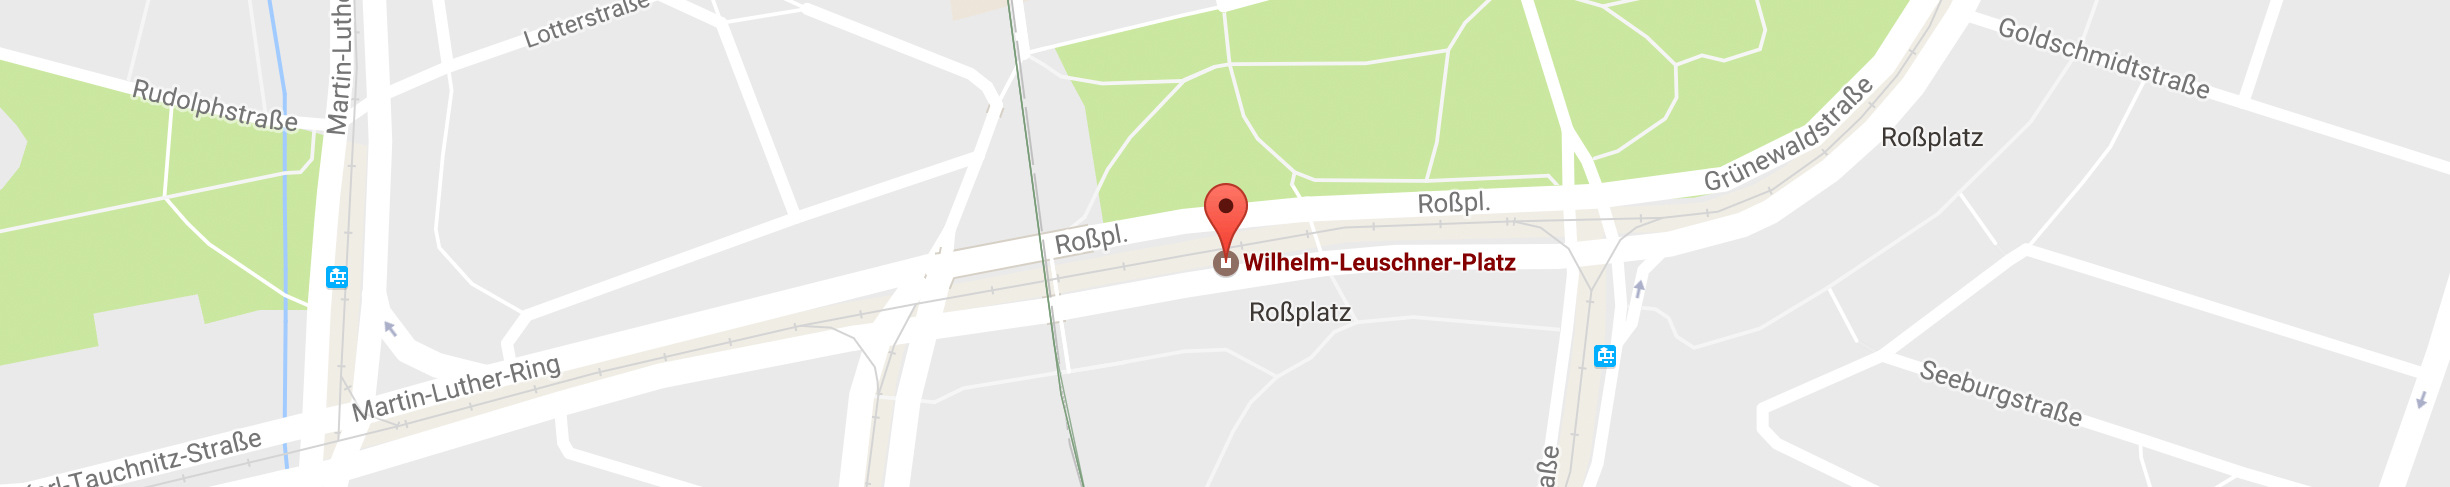
\includegraphics[width=\linewidth]{img/places/leuscher_map.jpg}
	\caption{Aufnahmeort City-Tunnel -- Wilhelm Leuschner Platz}
	\label{img:ak_map}
\end{figure}

	\subsubsection{Kameraeinstellungen}
	\begin{minipage}{0.58\textwidth}
		\begin{tabular}{ll}
			Kamera: &Canon EOS 7D \\
			Objektiv: &Canon EF 10-22mm \\
			& F/3.5-4.5 USM\\		
			Brennweite:& 12mm \\
			Belichtungszeit: & $\frac{1}{4}$s /$\frac{1}{2}$s / 1s / 2s / 4s\\
			Blendenwert: & f/8\\
			Empfindlichkeit & ISO 100 \\
		\end{tabular}\\
	\end{minipage}%
	\begin{minipage}{0.42\textwidth}
		\begin{figure}[H]
			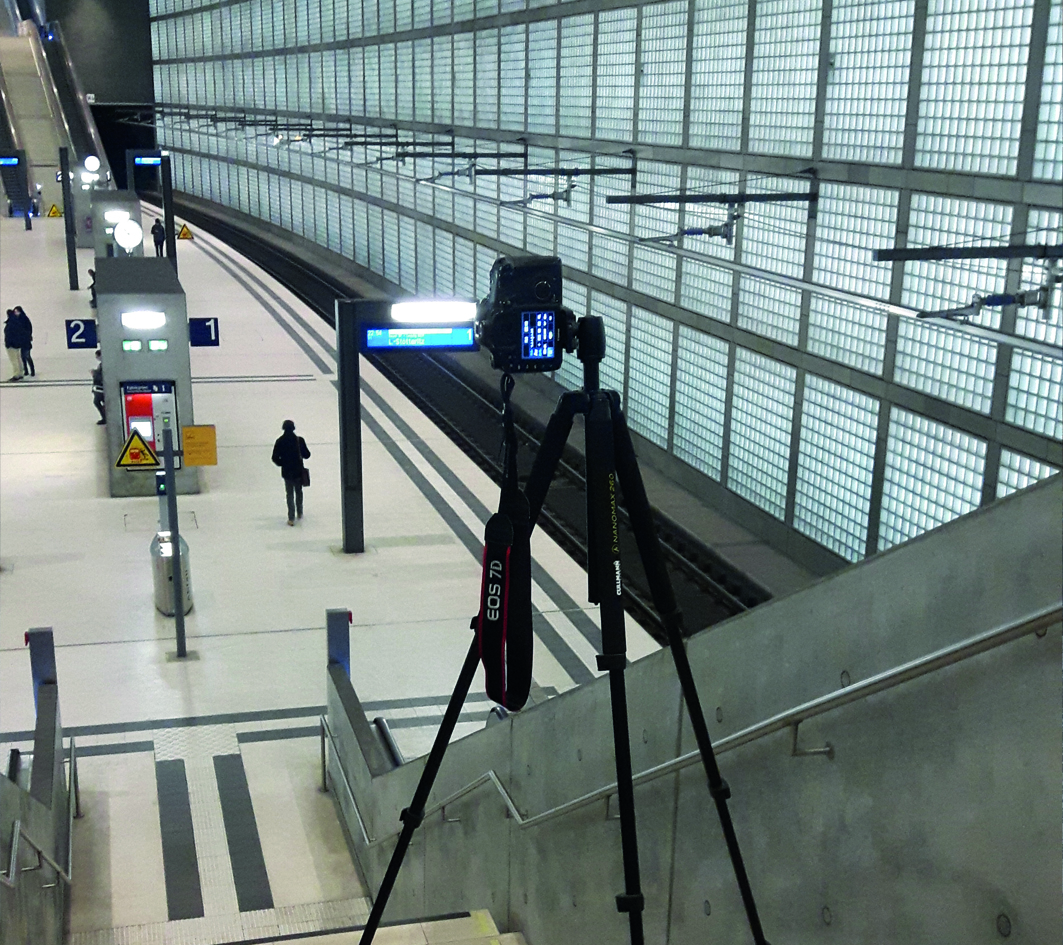
\includegraphics[width=\linewidth]{img/places/leuscher.jpg}
			\caption{Aufnahmesituation City-Tunnel}
			\label{img:ak}
		\end{figure}
	\end{minipage}%
		

	
	\subsubsection{Vorgehen}
	Die fünf Einzelbilder, welche später zu einem HDR-Foto zusammengefügt werden entstanden am 05.01.2017 um 23:21 Uhr. Es wurde versucht die Aufnahmen zu einem späten Zeitpunkt aufzunehmen um mögliche Störfaktoren wie beispielsweise einfahrende Züge oder umherlaufende Menschen zu minimieren. Auf Grund der langen Belichtungszeit erzeugen bewegte Objekte unscharfe Bildbereiche, sogenannte Geister, welche später zu Fehlern in der HDR-Fotografie führen. Die Kamera wurde am südlichen Eingang, oberhalb des Bahnsteigs, mittig platziert.

			 \newpage
			 \begin{figure}[h]
			 	
\includegraphics[width=\linewidth]{img/ph.jpg}
			 	\caption{HDR-Aufnahme City-Tunnel -- Wilhelm-Leuschner-Pl. }
			 \end{figure}


	\section{Deutsche Nationalbibliothek}
	\label{sec:bibo}
	\subsubsection{Aufnahmeort und -idee}
Die deutsche Nationalbibliothek hat innerhalb Deutschlands zwei Standorte und ist aus verschiedenen Einrichtungen hervorgegangen. Ihre Vorgänger waren die 1912 in Leipzig gegründete Deutsche Bücherei und die 1946 in Frankfurt a. M. gegründete Deutsche Bibliothek. Im Zuge der Wiedervereinigung wurden diese zu einer Institution zusammengelegt und 2006 zur Deutschen Nationalbibliothek umbenannt. 

\bigskip
Die Deutsche Nationalbibliothek hat den Auftrag alle deutschen und deutschsprachigen Publikationen ab 1913, im Ausland erscheinende deutsche Werke, Übersetzungen und zwischen 1933 und 1945 erschienene Werke deutschsprachiger Emigranten zu sammeln, archivieren und zu verzeichnen. 

\bigskip
Der moderne, halbrunde Anbau welche sich direkt an der Kreuzung Semmelweisstraße und Straße des 18. Oktober befindet, sticht durch seine besondere Architektur von der restlichen Umgebund heraus und bietet einen guten Kontrast zu dem historischen Teil der Leipziger Nationalbibliothek. Die indirekte Beleuchtung im Zusammenspiel mit den großen Glasfronten, macht es besonders in der Abendstunden zu einem sehr interessanten Motiv. 

\begin{figure}[H]
	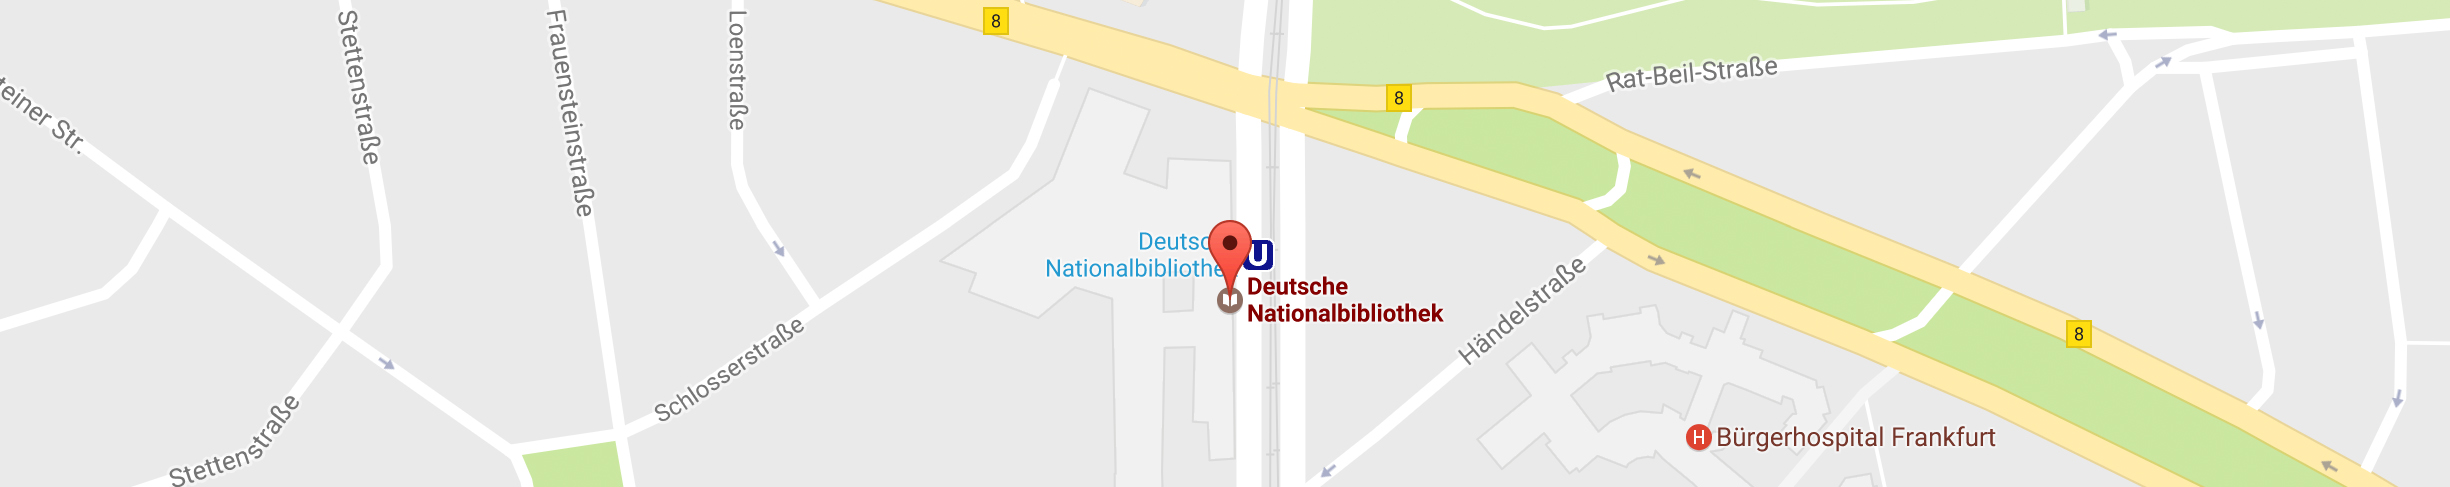
\includegraphics[width=\linewidth]{img/places/bibo_map.jpg}
	\caption{Aufnahmeort Deutsche Nationalbibliothek}
	\label{img:ak_map}
\end{figure}
	
	\subsubsection{Kameraeinstellungen}
	\begin{minipage}{0.58\textwidth}
		\begin{tabular}{ll}
			Kamera: &Canon EOS 7D \\
			Objektiv: &Canon EF 10-22mm \\
			& F/3.5-4.5 USM\\		
			Brennweite:&  \\
			Belichtungszeit: & \\
			Blendenwert: & \\
			Empfindlichkeit & \\
		\end{tabular}\\
	\end{minipage}%
	\begin{minipage}{0.42\textwidth}
		\begin{figure}[H]
			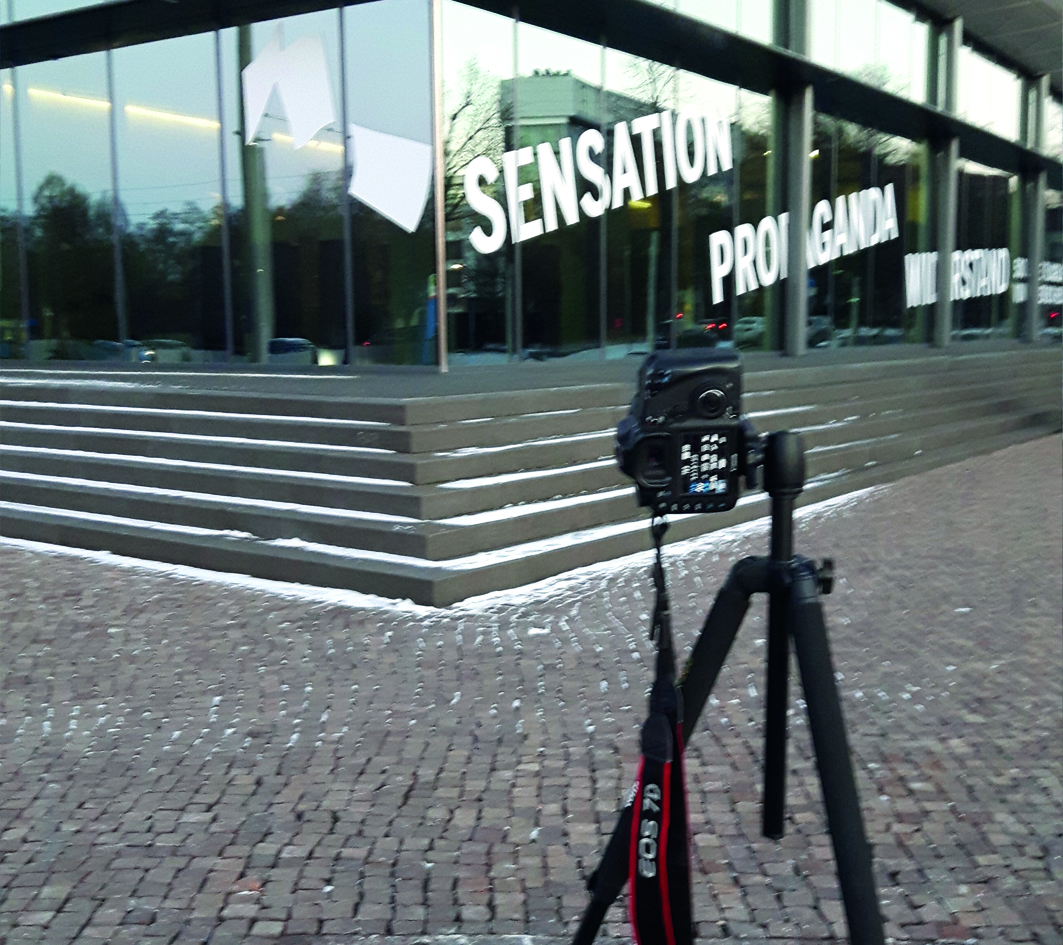
\includegraphics[width=\linewidth]{img/places/bibo.jpg}
			\caption{Aufnahmesituation Deutsche Nationalbibliothek}
			\label{img:ak}
		\end{figure}
	\end{minipage}%
			
	\subsubsection{Vorgehen}
	Die Kamera wurde mittig zur vorderen Ecke des modernen Anbaus positioniert und auf das Gebäude ausgerichtet. Auf Grund der vorherrschenden geraden Linien, der damit verbundenen Blickführung und der Verwendung eines Weitwinkelobjektivs entsteht eine schöne Zweipunktperspektive. Die fünf Einzelbilder wurden am 06.01.2017 um ?? aufgenommen. 
	
	
			 \newpage
			 \begin{figure}[h]
			 	
\includegraphics[width=\linewidth]{img/ph.jpg}
			 	\caption{HDR-Aufnahme Deutsche Nationalbibliothek}
			 \end{figure}

	

	
		\section{Speck's Hof}
	\label{sec:speck}
			\subsubsection{Aufnahmeort und -idee}
						Charakteristisch für die Leipziger Innenstadt, ist die Vielzahl an Passagen und Durchgangshöfen, welche das Stadtbild prägen. Die älteste, erhaltene Ladenpassage ist Speck\grq s Hof, welche zwischen 1908 und 1929, durch den Bau des Messehauses entstand. Den Namen erhielt die Passage auf Grund des Kaufhofes des Freiherrn von Speck, welches zuvor an dieser Stelle stand. Sie befindet sich an der Kreuzung Reichstraße / Grimmaische Straße, in direkter Nähe zur Nikolaikirche und ist mit dem Hansa Haus verbunden. In den Jahren 1993 bis 1995 wurde die Passage aufwendig restauriert. Heute bietet Speck\grq s Hof eine architektonische und gestalterische Mischung aus Vergangenheit und Moderne und ist beispielsweise durch Malereien und Plastiken der Künstler Bruno Griesel, Johannes Grützke und Moritz Götze verziert. Besonders ist den Abendstunden ist Speck's Hof von außen, durch eine indirekte Beleuchtung ein Blickfang. 

\begin{figure}[H]
	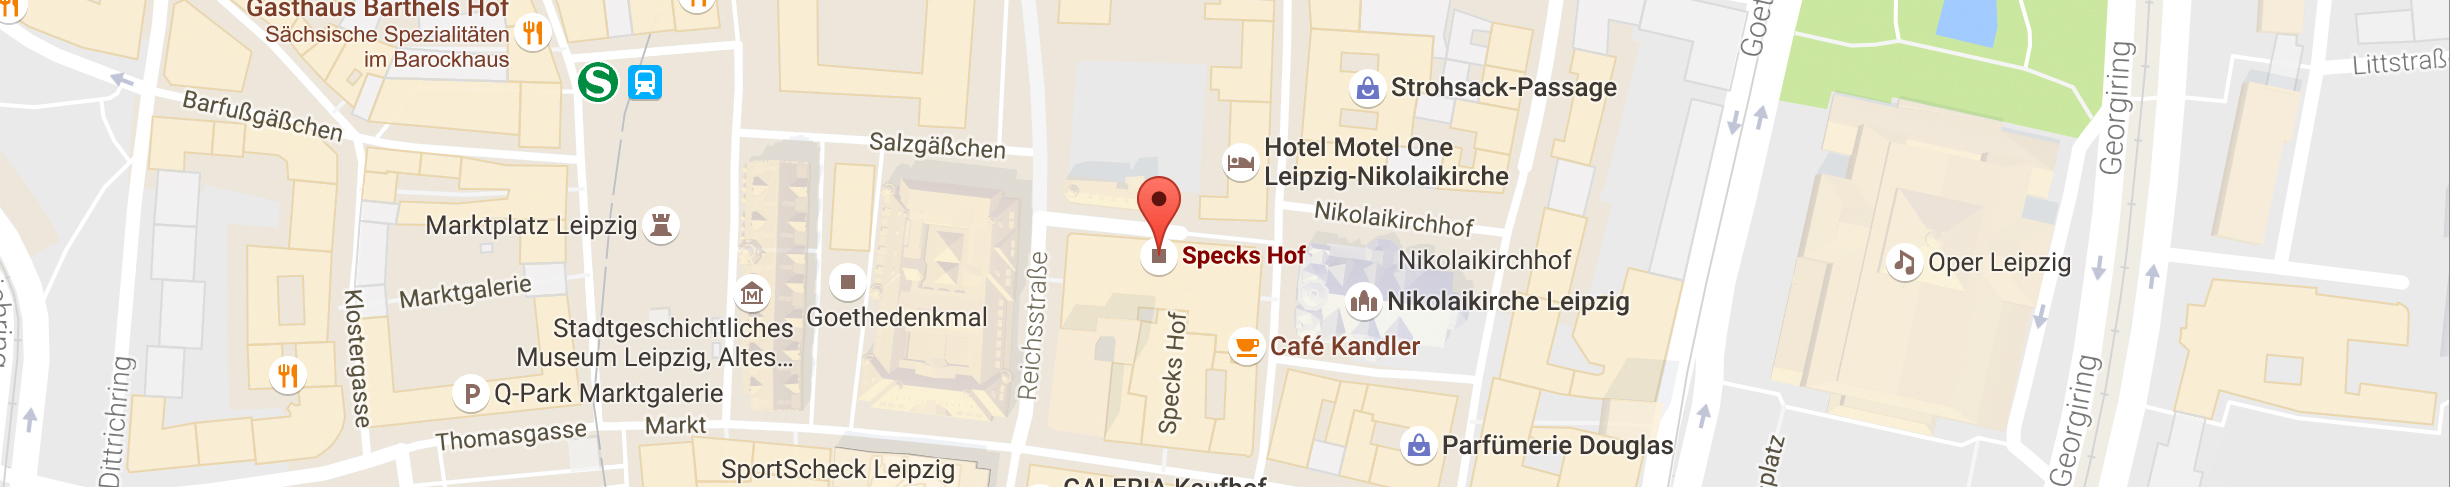
\includegraphics[width=\linewidth]{img/places/sh_map.jpg}
	\caption{Aufnahmeort Speck's Hof}
	\label{img:sh_map}
\end{figure}

\subsubsection{Kameraeinstellungen}
\begin{minipage}{0.58\textwidth}
	\begin{tabular}{ll}
		Kamera: &Canon EOS 7D \\
		Objektiv: &Canon EF 10-22mm \\
		& F/3.5-4.5 USM\\		
		Brennweite:&  10mm \\
		Belichtungszeit: &  \\
		Blendenwert: & \\
		Empfindlichkeit & \\
	\end{tabular}\\
\end{minipage}%
\begin{minipage}{0.42\textwidth}
	
\end{minipage}%
		
			
	\subsubsection{Vorgehen}
	Die Aufnahmen entstanden am 17.01.2017 um ?? während der Abend\-dämmerung, der sogenannten blauen Stunde. Ähnlich wie im Punkt 	\ref{sec:bibo} bereits beschrieben, wurde die Kamera an einer Ecke des Gebäudes platziert. Auch hier entsteht, durch die optische Linienführung, sowie die Verwendung eines Weitwinkelobjektivs eine Zweipunktperspektive. Im Zusammenspiel mit der besonderen, warmen Stimmung, welche durch die Kombination des künstlichen und des natürlichen Lichtes entsteht, macht den Reiz dieser  HDR-Aufnahme aus.
			
		
					 \newpage
					 \begin{figure}[h]
					 	
\includegraphics[width=\linewidth]{img/ph.jpg}
					 	\caption{HDR-Aufnahme Speck's Hof}
					 \end{figure}
			

	\chapter{Vorbereitung}
		Bei der HDR-Fotografie geht es im wesentlichen darum, den Kontrastumfang einer Szene vollständig abzubilden. Da der Dynamikumfang aktueller Kameras beschränkt ist, erfordern spezielle Situationen den Einsatz dieser Technik. Das bedeutet, dass vom selben Motiv, mehrere Fotos mit unterschiedlichen Belichtungszeiten zu erzeugen sind. Diese werden in der Nachbearbeitung zu einem einzigen Bild zusammengefasst, welches nun einen erhöhten Dynamikumfang besitzt. Sinnvolle Motive für diese Technik können z. B. Innenaufnahmen, Nachtaufnahmen oder Gegenlichtaufnahmen sein.
		
		\bigskip
		Für die Aufnahme mehrerer Einzelbilder, ist es ratsam ein Stativ zu verwenden, um Verwacklungen auszuschließen. Auch ist bei Nachtaufnahmen besonders auf variierende Lichtsituationen zu achten, da z. B. Fahrradfahrer in der Langzeitbelichtung unschöne Lichtstreifen hinterlassen.
	
	\section{Einzelbildaufnahmen}
	\label{sec:einzel}
		Für die Erstellung der Einzelbildaufnahmen, besitzt die in dieser Arbeit verwendete Canon 7D die sog. Bracketing-Funktion. Diese ist dafür zuständig, automatisierte Belichtungsreihen zu erstellen. Für die besagte Kamera gibt es eine inoffizielle Erweiterung namens \grqq{}Magic Lantern\grqq{} (http://www.magiclantern.fm), welche sie überwiegend an Filmer richtet. Dennoch besitzt sie auch ein Menüpunkt für Fotografen und ermöglicht u. a. Belichtungsreihen bestehend aus bis zu 13 Fotos.
		
		\bigskip
		Diese Funktion erstellt ein normal belichtetes Foto, gefolgt von jeweils 2 über- und unterbelichteten Aufnahmen. Die dafür verwendete Schrittweite lässt sich in Lichtwerten (engl. Exposure Value EV) einmalig einstellen, wobei die folgenden Einstellungsmöglichkeiten vorhanden sind: 0.5, 1, 1.5, 2, 3, ..., 8. Jede Erhöhung/Verringerung des Lichtwertes um eins, bedeutet die Halbierung/Verdopplung der Belichtung. 


	\chapter{HDR-Erstellung}
	\label{ch:processing}
		Nach dem Erstellen der Belichtungsreihen, werden die Einzelbilder mit einer entsprechenden Software zu einem HDRI (High Dynamic Range Image) zusammengesetzt. Dieses besitzt einen erhöhten Dynamikumfang und liegt deshalb im 32-Bit-Format vor. Der Vorteil liegt darin, dass dieser dafür genutzt werden kann, unter- oder überbelichtete Aufnahmen korrekt zu belichtet. Dieser Schritt nennt sich \textit{Tone-Mapping}.
		Da aktuelle Drucker und Bildschirme diesen Dynamikumfang nicht darstellen können, erzeugt die verwendete Software zum Abschluss ein runtergerechnetes 8-Bit-Bild. Dieses wird auch LDR-Bild (Low Dynamic Range) genannt 
		
		\bigskip
		Die Kapitel \ref{sec:photoshop} und \ref{sec:photomatix} behandeln den Prozess des Tone-Mappings am Beispiel zweier Softwarelösungen.

	
	\section{Adobe Photoshop Lightroom}
	\label{sec:photoshop}
		Adobe Lightroom wird von vielen Fotografen zum Verwalten und Bearbeiten ihrer Fotos verwendet. Dabei speichert dieses Programm alle Bearbeitungsschritte und wendet diese erst beim Export auf das Bild an. Dadurch lassen sich Änderungen jeder Zeit rückgängig machen und die Originaldatei bleibt unberührt. Dennoch erzeugt es eine Live-Vorschau der aktuellen Änderungen. Auch unterstützt es die HDR-Erstellung, welche in dieser Arbeit dennoch nicht zum Einsatz kommt. Ferne wird hier in Kombination mit Photoshop HDR Pro gearbeitet, da dieses garantiert ein 32-Bit-Bild erstellt.
		
		\bigskip
		Dazu wählt man nach dem Import in Lightroom eine Belichtungsreihe aus. Anschließend kann über das Kontextmenü, unter dem Menüpunkt \textit{Bearbeiten in > In Photoshop zu HDR Pro zusammenfügen}, der RAW-Editor von Photoshop mit den markierten Aufnahmen geöffnet werden (s. Abb. \ref{img:light_1}).
		
		\bigskip
		\begin{figure}[H]
			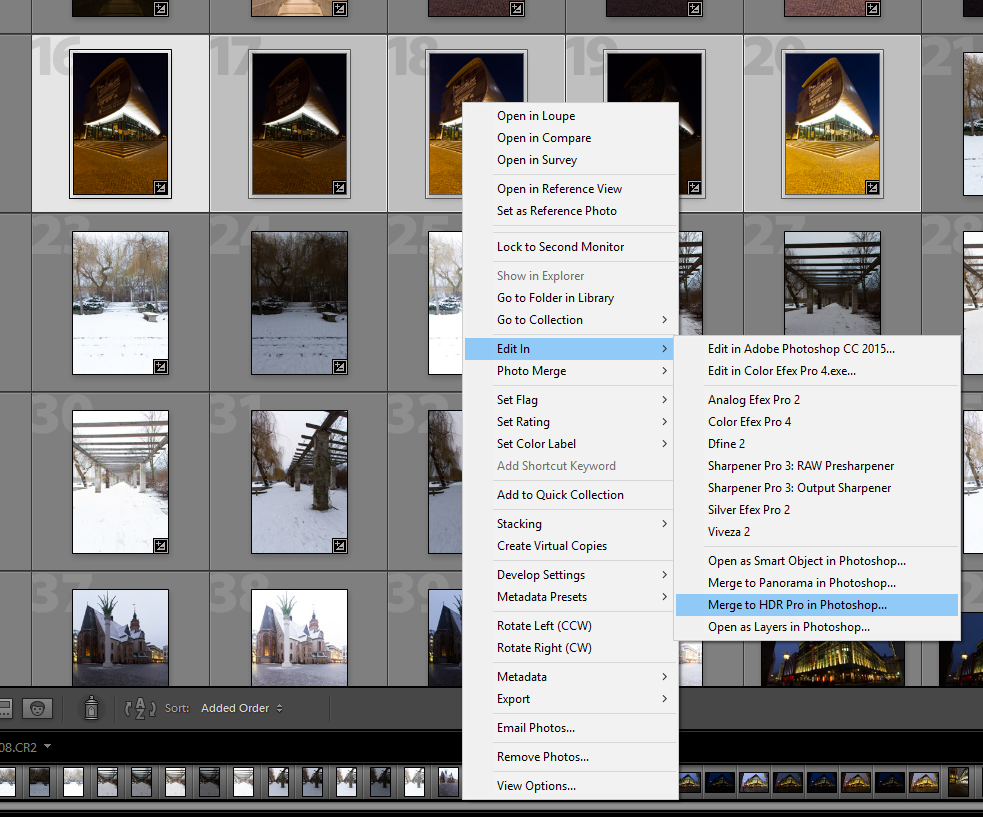
\includegraphics[width=\linewidth]{img/lightroom1.png}
			\caption{Lightroom - Belichtungsreihe und Klickpfad}
			\label{img:light_1}
		\end{figure}
	
		Im darauf folgenden Fenster lässt sich der Dynamikumfang des Zielbildes einstellen, wobei für diese Arbeit 32-Bit gewählt werden. Zusätzlich lassen sich sog. Geister entfernen. So werden Schemenhafte Darstellungen von sich bewegenden Objekten genannt, die sich zwischen den Einzelbildern an unterschiedlichen Positionen befinden. Die Software bestimmt im Anschluss eines der importierten Fotos und korrigiert das Zielbild dementsprechend. Der Benutzer kann an dieser Stelle auch manuell Eingreifen und ein Foto mit möglichst wenig Bewegung auswählen (s. Abb. \ref{img:light_2}). Mit einem klick auf \textit{OK}, wird das erzeugte Foto in Photoshop geöffnet. Anschließend kann das Programm geschlossen werden, wobei der aufploppende Speicherdialog bestätigt werden muss. Dies leitet das Speichern des Fotos im tiff-Format ein. Lightroom erkennt das neue Foto und lädt es automatisch in die aktuelle Bibliothek rein, wo es anschließend bereit für die Bearbeitung ist.
		
		\bigskip
		\begin{figure}[H]
			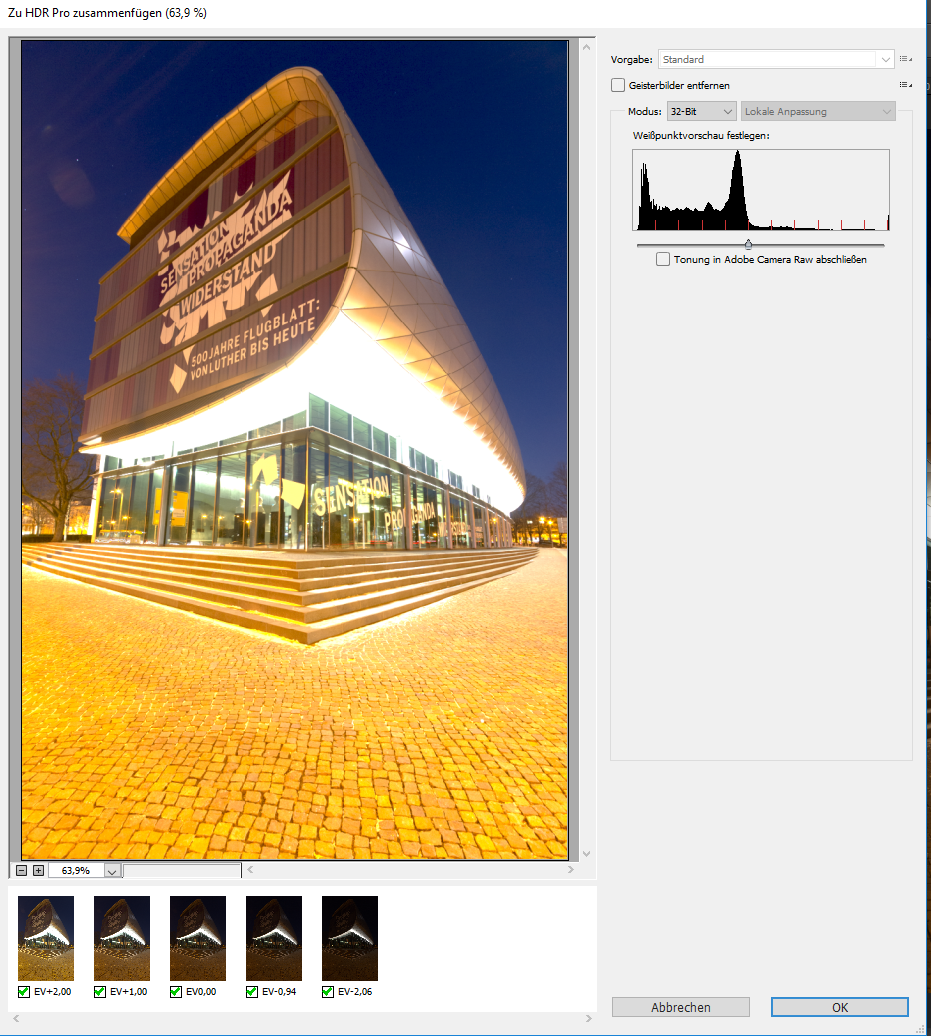
\includegraphics[width=.95\linewidth]{img/lightroom2.png}
			\caption{Lightroom - Photoshop Pro HDR-Entwicklung}
			\label{img:light_2}
		\end{figure}
		
		Lightroom bietet keine zusätzlichen Bearbeitungsfunktionen speziell für HDR, weshalb mit dieser Software gut realistisch wirkende LDR-Bilder erstellt werden können. Zur Verfügung stehen alle gängigen Einstellungsmöglichkeiten für die Fotonachbearbeitung s. Abb. \ref{img:light_3}.
		
		\bigskip
		\begin{figure}[H]
			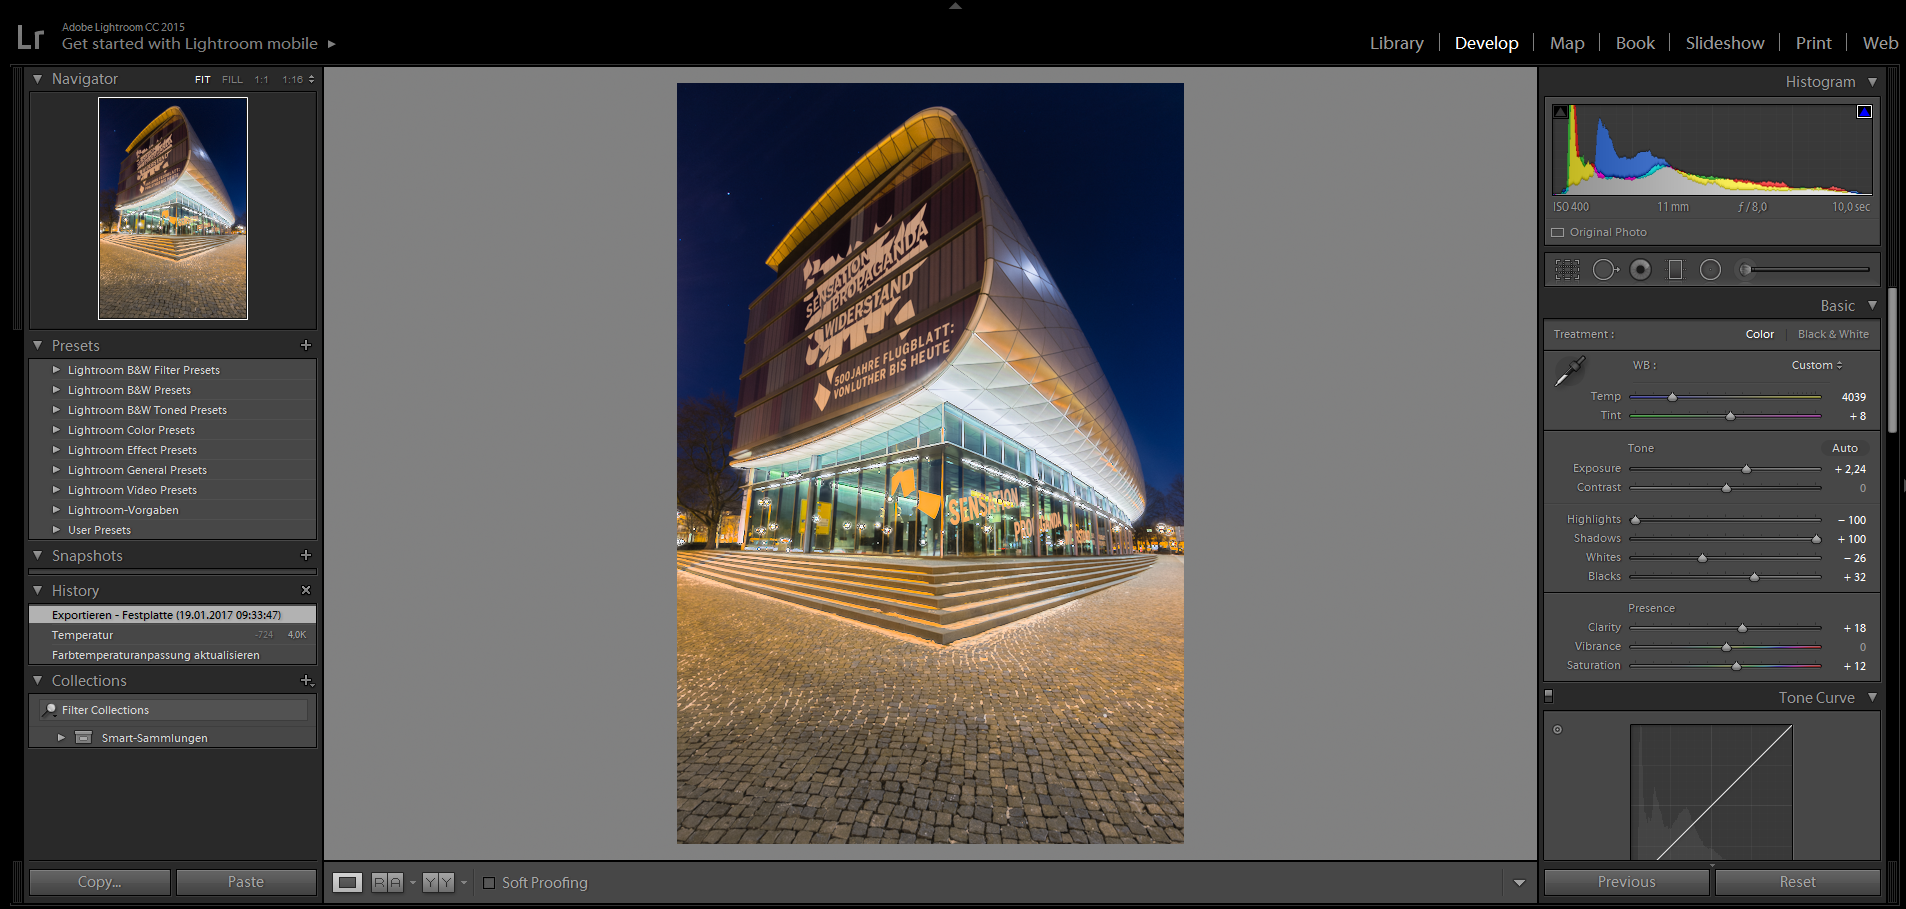
\includegraphics[width=\linewidth]{img/lightroom3.png}
			\caption{Lightroom - Erstelltes HDR und Einstellungsmöglichkeiten}
			\label{img:light_3}
		\end{figure}
	
	\section{Photomatix}
	\label{sec:photomatix}
		Im Gegensatz zu Lightroom (\ref{sec:photoshop}), liegt das Spezialgebiet der Software Photomatix auf HDR-Entwicklung. Bei der Installation ist es sogar möglich ein zusätzliches Plugin für Lightroom zu installieren, um Belichtungsreihen aus dieser Software heraus in Photomatix zu importieren und bearbeitete Bilder in Lightroom zu öffnen.
		
		Als erstes muss eine Belichtungsreihe geladen werden, wobei im anschließenden Fenster diverse Optionen für das Zusammenfügen vorhanden sind (s. Abb. \ref{img:photo2}). Die Bilder können automatisch ausgerichtet, Geisterbilder entfernt, Rauschen reduziert und Chromatische Aberrationen reduziert werden. Da alle Fotos mit Hilfe eines Stativs aufgenommen sind, müssen diese nicht ausgerichtet werden. Es ist sinnvoll chromatische Aberrationen zu entfernen.
		
		\bigskip
		\begin{figure}[H]
			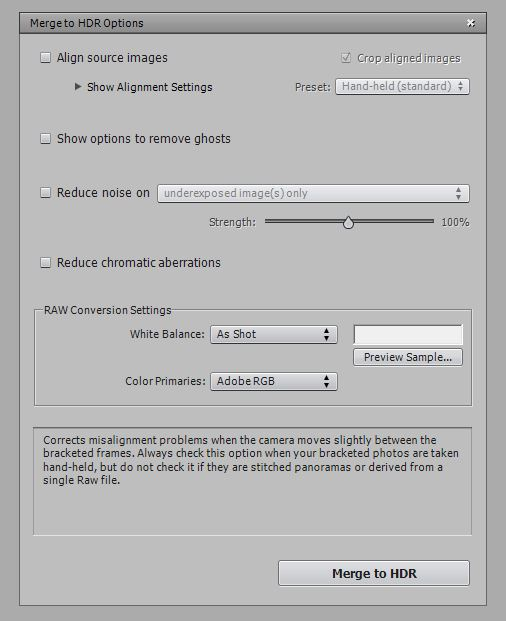
\includegraphics[width=0.8\linewidth]{img/photo2.jpg}
			\caption{Photomatix - Zusammenführen zu HDR}
			\label{img:photo2}
		\end{figure}
	
		Nachdem das HDR-Bild erstellt ist, gibt es 3 Möglichkeiten das erzeugte Bild mittels spezieller Tone-Mapping-Methoden zu bearbeiten. Diese sind \textit{Contrast Optimizer}, \textit{Tone Compressor} und \textit{Detail Enhancer} und werden im Folgenden exemplarisch erläutert. Die dargestellten Ergebnisse sind jeweils überspitzt dargestellt und wirken wenig fotorealistisch.
		
		\bigskip
		\paragraph{Contrast Optimizer} Diese Methode ist speziell dafür gedacht, die Darstellung von Kontrasten zu optimieren. Mit den folgenden Schiebereglern lässt sich das HDR-Bild bearbeiten: Stärke, Tonwertkompression,	Lichtwirkung, Weißpunkt, Schwarzpunkt, Mitteltöne, Farbsättigung und Farbtemperatur (siehe Abbildung \ref{img:photo4}). Wie der Name der Methode schon vermuten lässt, werden mit diesen Einstellungen die Hell-Dunkel-Kontraste stark berücksichtigt, sodass Die Farbsättigung angehoben werden muss.
		
		\bigskip
		\begin{figure}[H]
			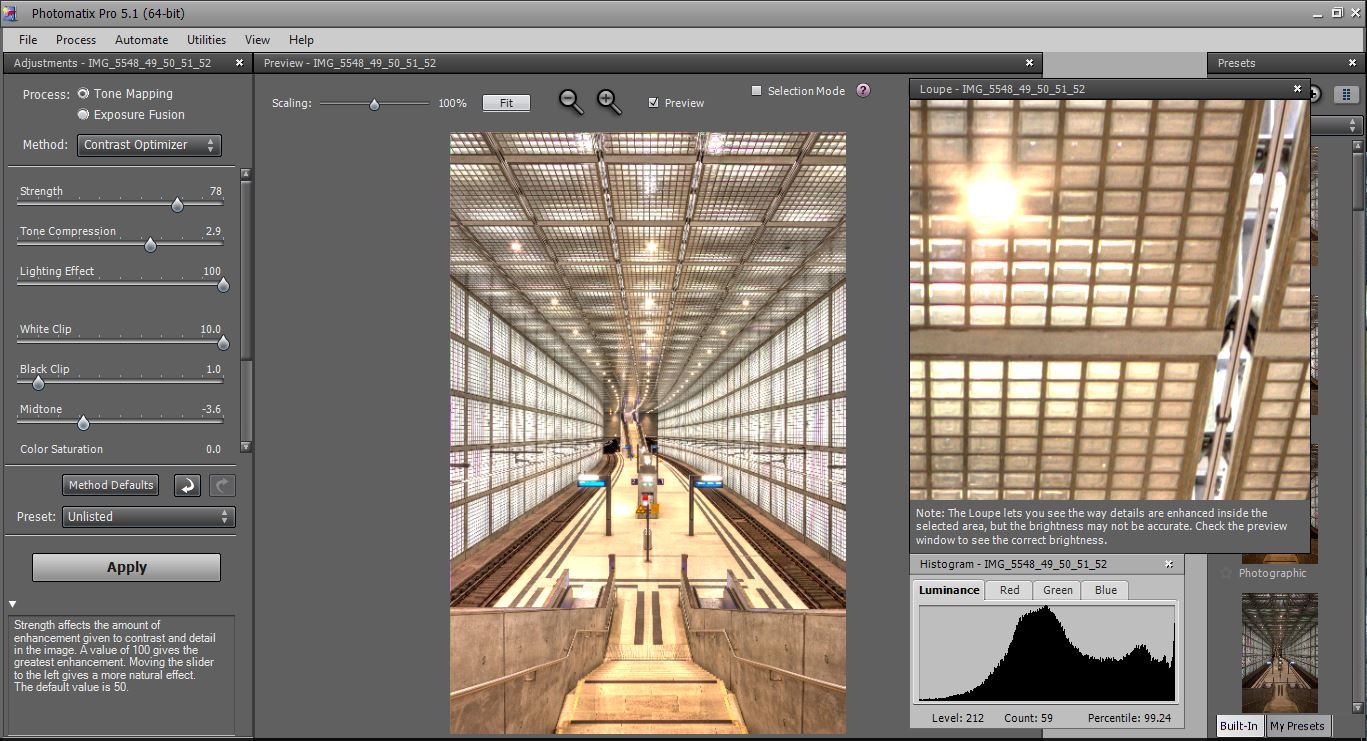
\includegraphics[width=\linewidth]{img/photo4.jpg}
			\caption{Photomatix - Contrast Optimizer}
			\label{img:photo4}
		\end{figure}
		
		\paragraph{Tone Compressor} Im Gegensatz zu der vorherigen Methode kann dieses Mal mehr Einfluss auf die Farben genommen werden. Dies implizieren Reglernamen wie Helligkeit, Tonwertkompression, Kontrastanpassung, Weißpunkt, Schwarzpunkt, Farbsättigung und Farbtemperatur. Dafür ist es schwer möglich den Hell-Dunkel-Kontrast zu optimieren. Die Abbildung \ref{img:photo5} veranschaulicht dies gut. Der Schwarzpunkt ist bereits auf das Minimum reduziert, trotzdem sind nur wenig Details in den Schienen zu erkennen. Der Fokus liegt offenbar auf dem erweiterten Farbraum des HDR-Bildes, wodurch ein oftmals surreales Resultat entsteht.
		
		\bigskip
		\begin{figure}[H]
			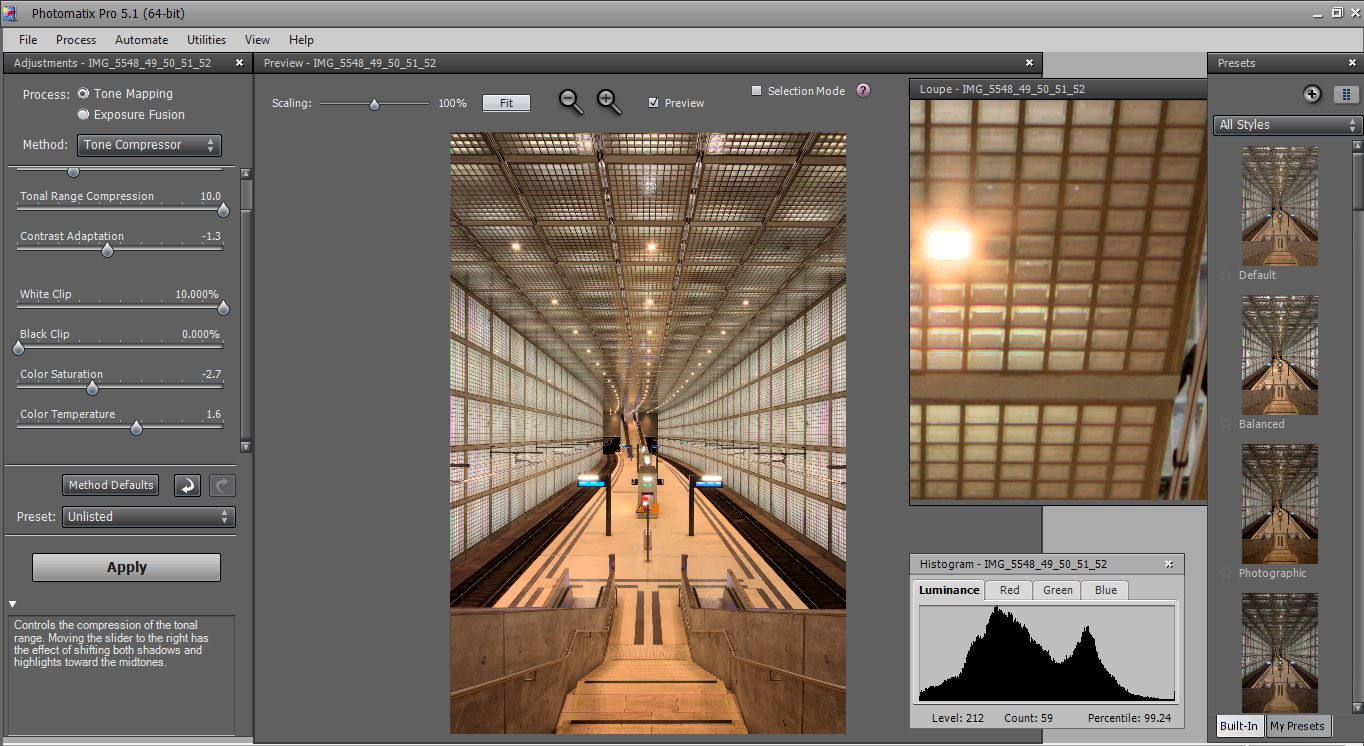
\includegraphics[width=\linewidth]{img/photo5.jpg}
			\caption{Photomatix - Tone Compressor}
			\label{img:photo5}
		\end{figure}
	
		\paragraph{Detail Enhancer} In diesem Modus können zu den bereits erwähnten Einstellungsmöglichkeiten der beiden anderen Modi, zusätzlich noch Detailskontrast und Lichteffekte definiert werden. Wie in Abbildung \ref{img:photo3} zu sehen ist, gibt es vorgefertigte Presets für die Lichtwirkung. In dieser Abbildung wurde der maximale surreal Wert verwendet, was dem Foto den bekannten HDR-Effekt verleiht.
		In diesem Modus kann sehr gut Einfluss auf Farb- und Kontrasteinstellungen genommen werden, wodurch er sich besonders gut für die HDR-Entwicklung in Photomatix eignet. 
		
		\bigskip
		\begin{figure}[H]
			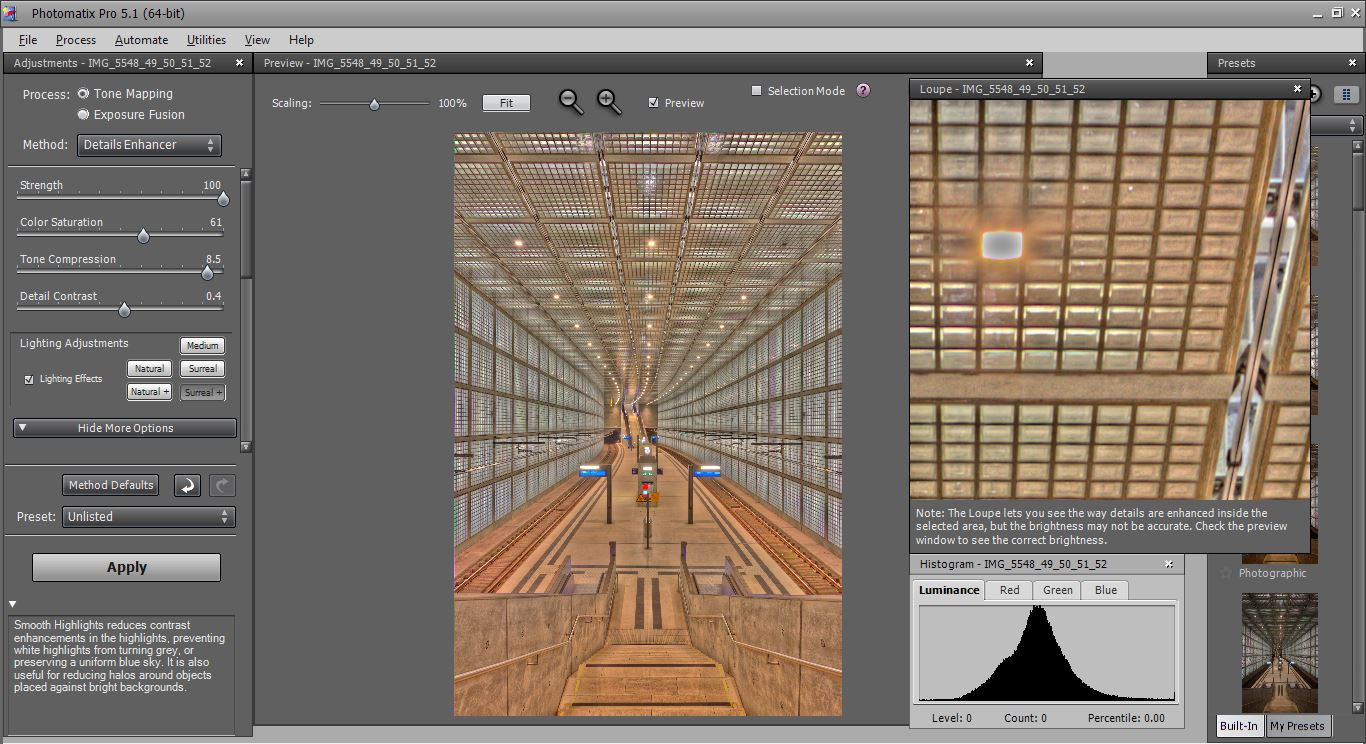
\includegraphics[width=\linewidth]{img/photo3.jpg}
			\caption{Photomatix - Detail Enhancer}
			\label{img:photo3}
		\end{figure}
	
		Es können sehr surreal wirkende Fotos erstellt werden, realitätsnahe Bilder sind mit entsprechenden Einstellungen auch möglich. Das liegt auch daran, dass es weitere Einstellungsmöglichkeiten unter den Punkten \grqq{}Show more options\grqq{} und \grqq{}Show advanced options\grqq{} gibt. Diese sind: Lichter glätten, Weißpunkt,	Schwarzpunkt, Gamma, Farbtemperatur, Mikrokontraste glätten, Sättigung Lichter, Sättigung Schatten, Schatten glätten und Schatten beschneiden (s. Abb. \ref{img:photo6}).
		
		\bigskip
		\begin{figure}[H]
			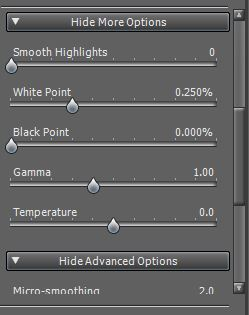
\includegraphics[width=.5\linewidth]{img/photo6.jpg}
			\caption{Photomatix - Detail Enhancer Optionen}
			\label{img:photo6}
		\end{figure}
	
	\chapter{Nachbearbeitung}
	\label{ch:nach}
		Durch den Fotomerge mit Photoshop kommt es manchmal, beim Versuch der Entfernung von Lichtstreifen, zu unschönen Konturen. Die Abbildung \ref{img:bibo_normal} veranschaulicht dieses Phänomen anhand des Fotos der Deutschen Nationalbibliothek. Im letzten Foto sind Autos in der Spiegelung zu sehen. Um dieses Problem zu lösen, kann man das entsprechende Foto entweder weglassen oder die Streifen durch die Originaldatei zurückersetzen.
		\bigskip
		\begin{figure}[H]
			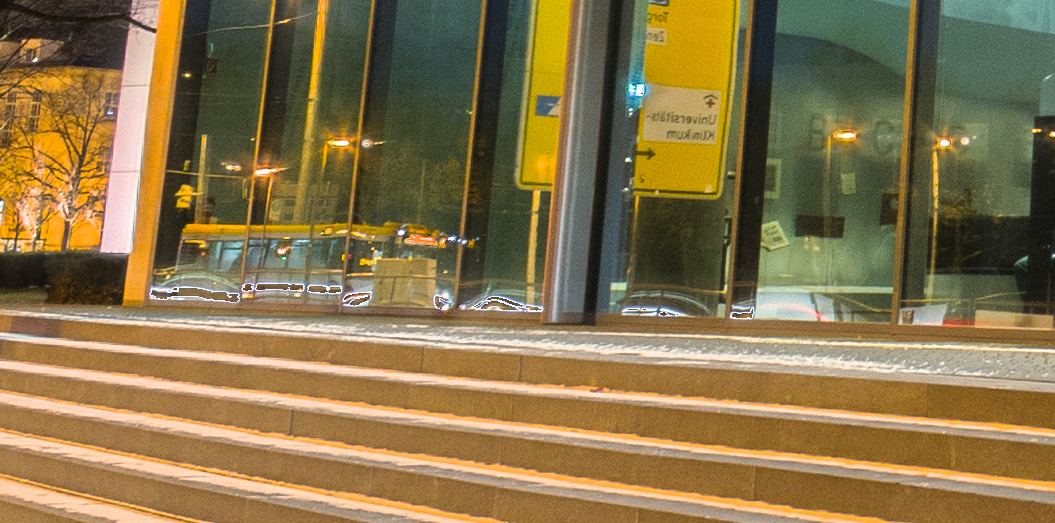
\includegraphics[width=\linewidth]{img/bibo_unbearbeitet.PNG}
			\caption{Nachbearbeitung - Bibliothek mit Lichtstreifen}
			\label{img:bibo_normal}
		\end{figure}
		
		Die Abbildung \ref{img:bibo_reworked} zeigt, wie die Problemstelle nach der Bearbeitung aussieht.
		\bigskip
		\begin{figure}[H]
			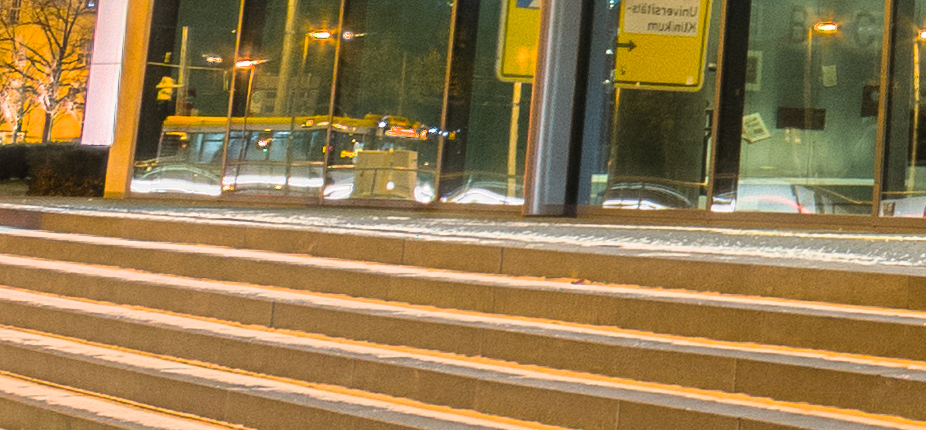
\includegraphics[width=\linewidth]{img/bibo_bearbeitet.PNG}
			\caption{Nachbearbeitung - Bibliothek ohne Lichtstreifen}
			\label{img:bibo_reworked}
		\end{figure}
		
		Bei der Aufnahme der Nikolaikirche ist ein Radfahrer durchs Bild gefahren und hat vereinzelt Lichtstreifen ins Bild gezaubert. Die Abbildung \ref{img:stamp} zeigt, wie dieser Streifen weggestempelt wird. Auch störende Schneestreifen oder Müll werden in jedem Bild berücksichtigt und gestempelt.
		
		\bigskip
		\begin{figure}[H]
			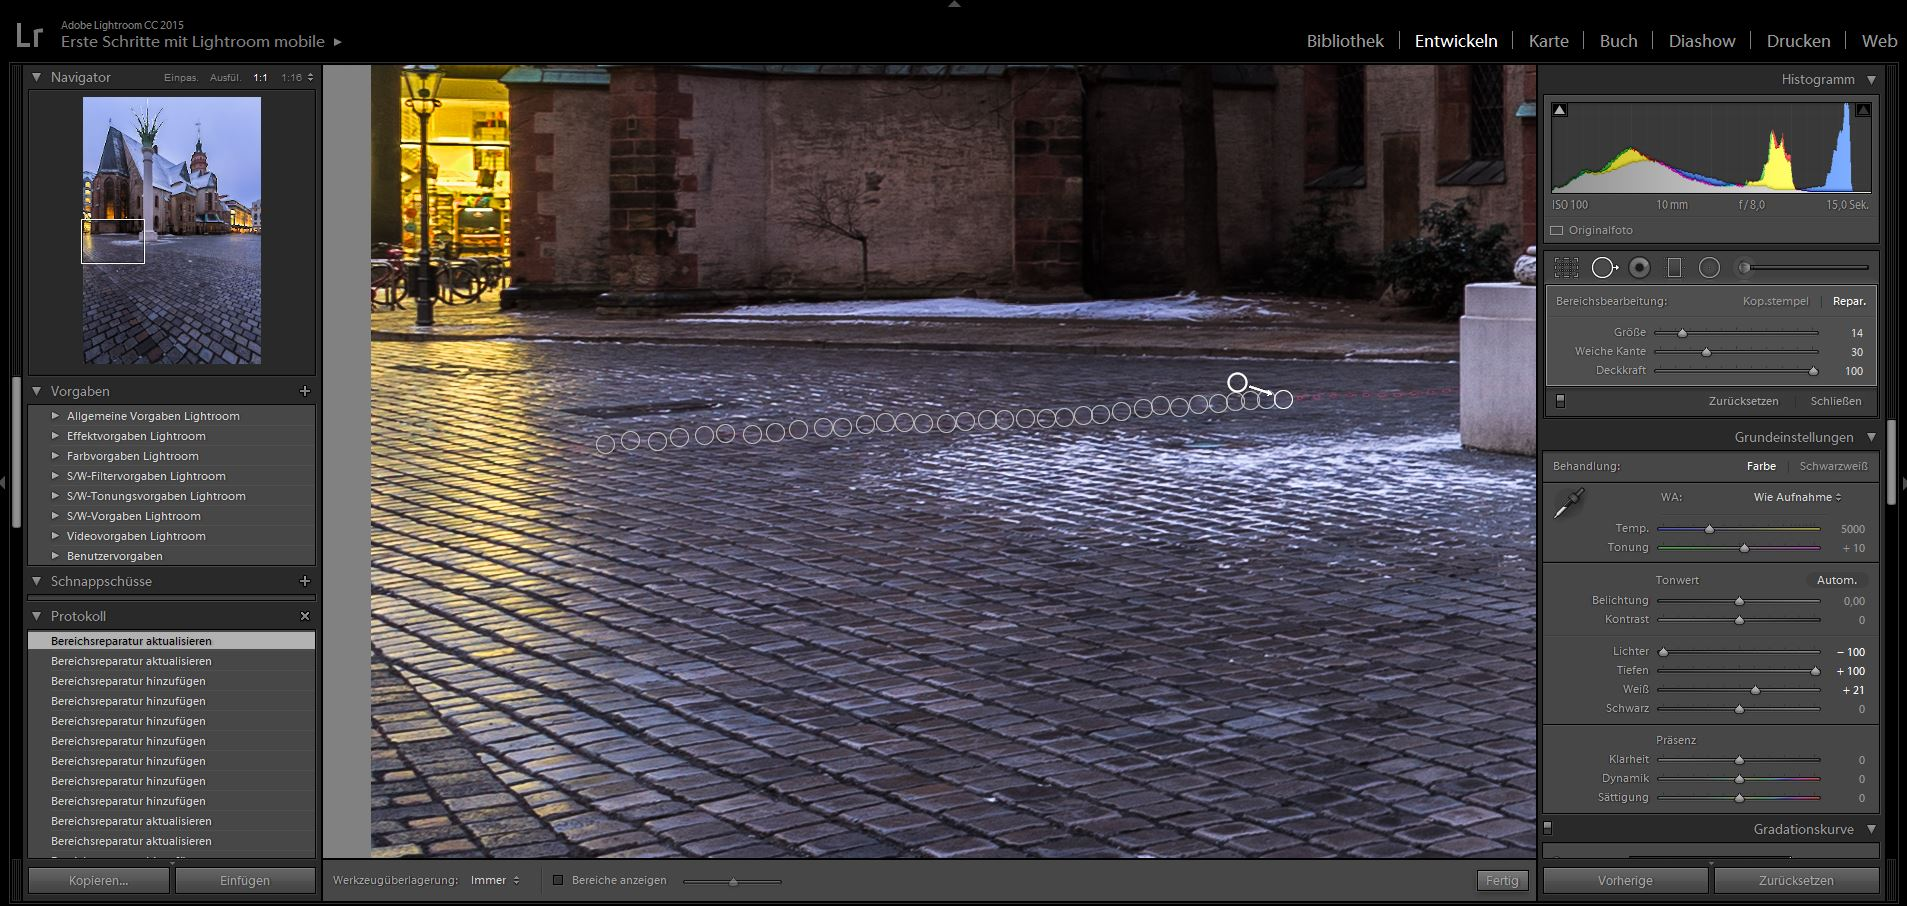
\includegraphics[width=\linewidth]{img/hdr_stempeln.JPG}
			\caption{Nachbearbeitung - Stempeln}
			\label{img:stamp}
		\end{figure}
	
\end{document}